\section{Nachbesserung eines Pfads}
Neben den im vorherigen Abschnitt beschriebenen Überkreuzungen kommt es bei den generierten Graphen auch zu solchen, die durch ein einfaches umlegen der Route verbessert werden können.

\begin{figure}[h]
    \begin{center}
    \caption{Graph vor und nach der Nachbesserung}
    \label{fig:after-control-ex1}
    \subfloat[Verbesserungsfähiger Graph \label{subfig:after-control-ex1-1}]{
        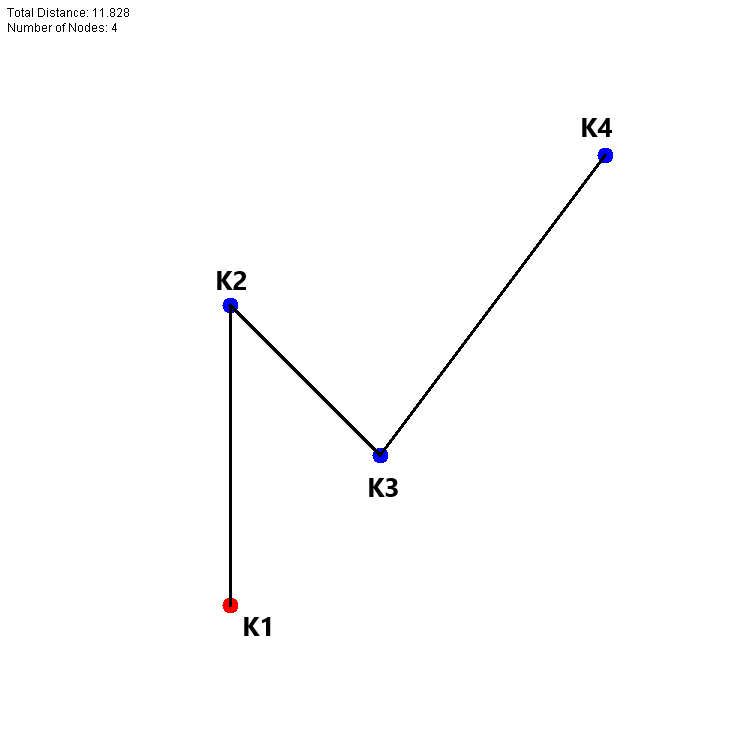
\includegraphics[width=0.35\textwidth]{Bilder/afterControl/after_control_ex1.PNG}
    }
    \hfil
    \subfloat[Verbesserter Graph \label{subfig:after-control-ex1-2}]{
        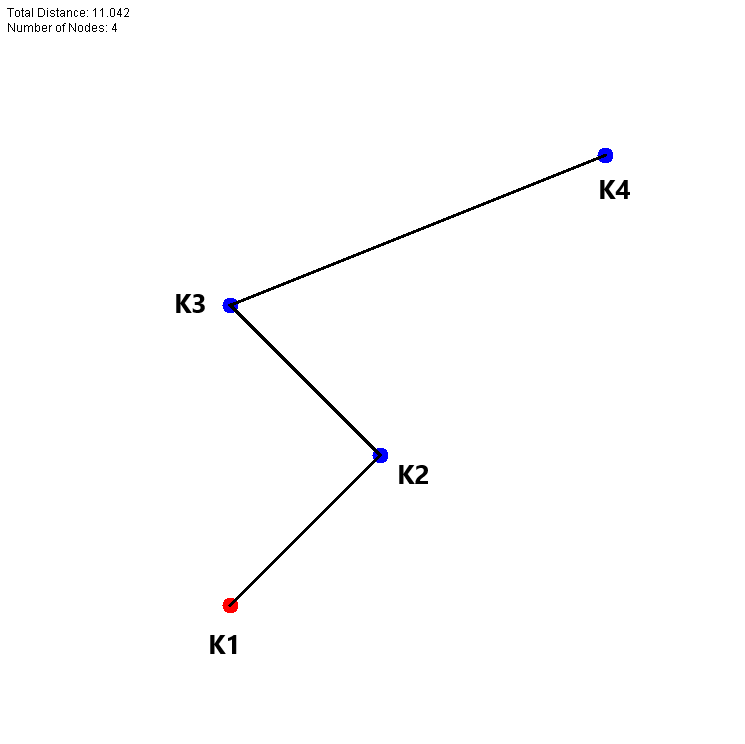
\includegraphics[width=0.35\textwidth]{Bilder/afterControl/after_control_ex2.PNG}
    }
    \end{center}
\end{figure}

Das Beispiel in \vref{fig:after-control-ex1} zeigt einen Graphen mit einer initialen Knotenreihenfolge
$$P = k_1,k_2,k_3,k_4$$
Durch das Umlegen zu
$$P =k_1,k_3,k_2,k_4$$
erfolgt eine Verringerung der Gesamtdistanz.
Betrachtet man die hier betroffenen Kanten $(k_1,k_2)$, $(k_1,k_3)$ und $(k_2,k_3)$ kann die Distanzverringerung anhand ihrer einzelnen Distanzen und ihres Auftretens in den beiden Graphen erklärt werden.
